\begin{figure}[t]
    \centering
    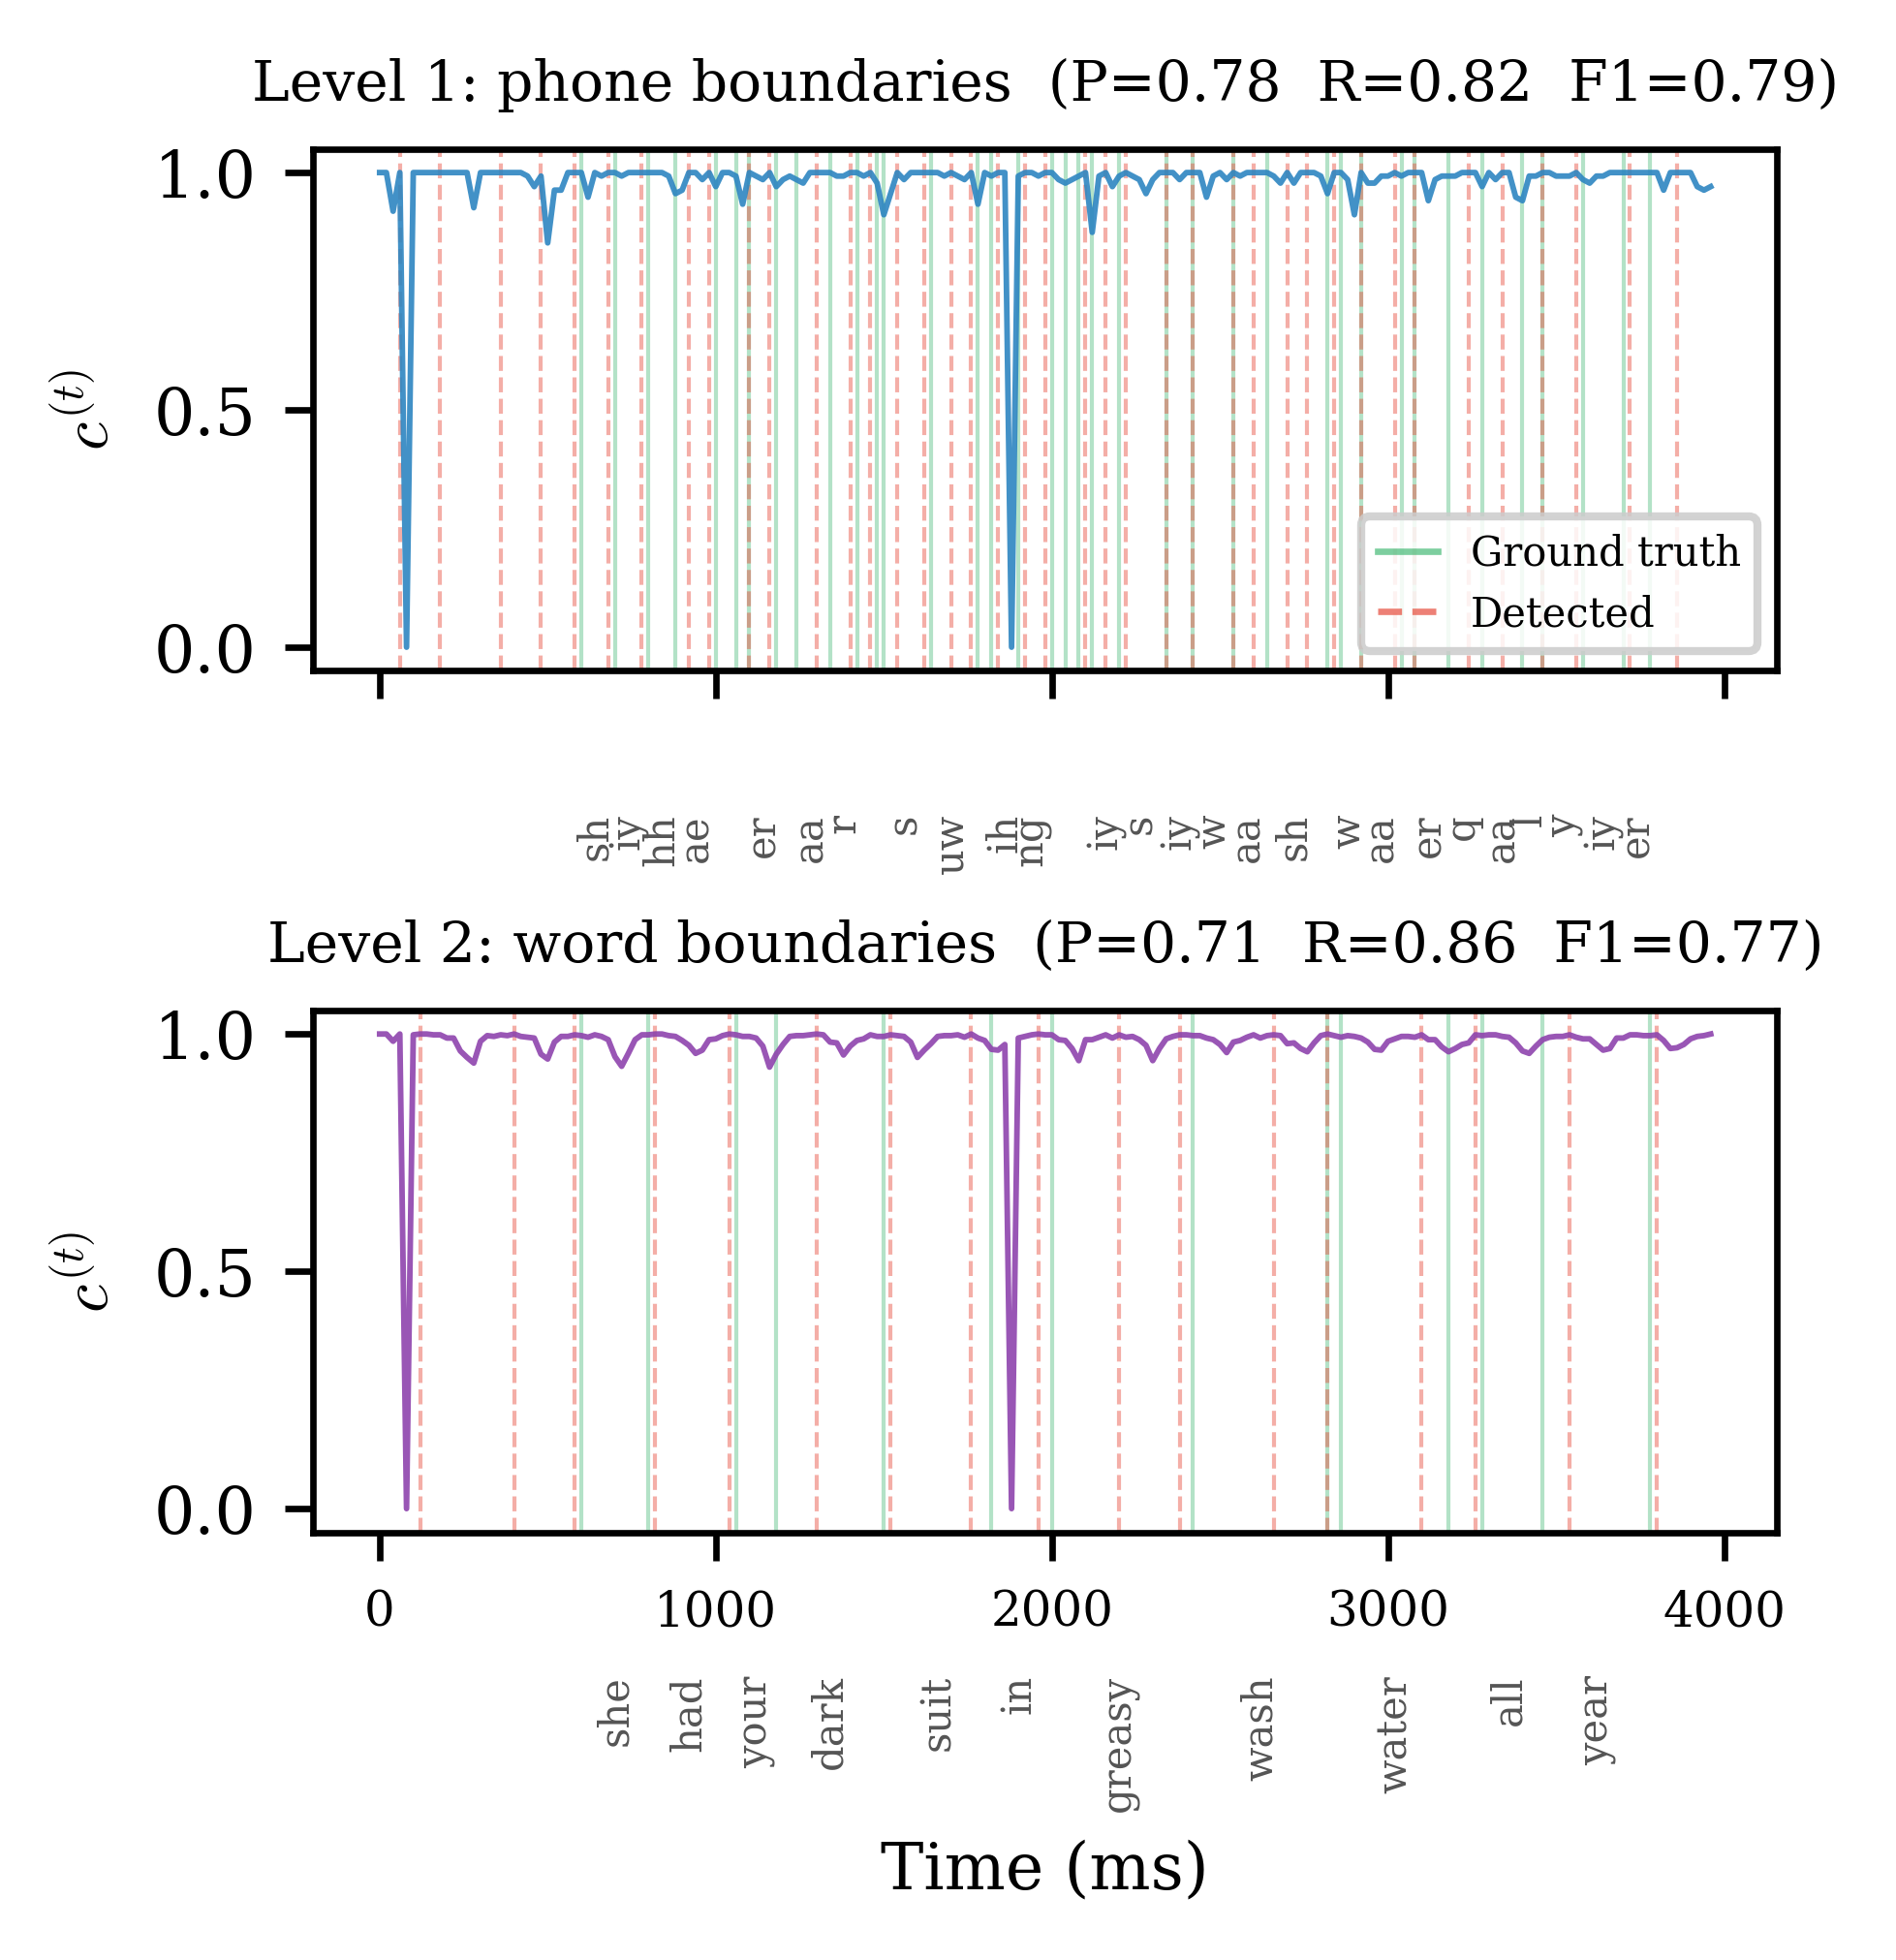
\includegraphics[width=0.9\columnwidth]{figures/boundary_signal.png}
    \caption{Assembly change signal $c^{(t)}$ (Eq.~\ref{eq:change}) for a single TIMIT utterance. \textbf{Top:} Level~1 (phone boundaries). \textbf{Bottom:} Level~2 (word boundaries). Green vertical lines mark ground-truth boundaries; red dashed lines mark detected peaks. Phone/word labels are shown below each axis.}
    \vspace{-10pt}
    \label{fig:boundary_signal}
\end{figure}
